%Canonical_Forms.tex
%
% Homework on Canonical Forms
% Frank Sottile
%%%%%%%%%%%%%%%%%%%%%%%%%%%%%%%%%%%%%%%%%%%%%%%%%%%%%%%%%%%%%%%%%%%%%%%
\documentclass[12pt]{article}
\usepackage{multicol,amssymb,amsmath}
\usepackage{graphicx}
\usepackage{xcolor}
\headheight=8pt
%
\topmargin=-95pt
\textheight=744pt   \textwidth=575pt
\oddsidemargin=-60pt \evensidemargin=-60pt

\pagestyle{empty}

%%%%%%%%%%%%%%%%%%%%%%%%%%%%%%%%%%%%%%%%%%%%
\newcommand{\HH}{{\mathbb H}}
\newcommand{\FF}{{\mathbb F}}
\newcommand{\RR}{{\mathbb R}}
\newcommand{\CC}{{\mathbb C}}
\newcommand{\KK}{{\mathbb K}}
\newcommand{\NN}{{\mathbb N}}
\newcommand{\QQ}{{\mathbb Q}}
\newcommand{\TT}{{\mathbb T}}
\newcommand{\ZZ}{{\mathbb Z}}
\newcommand{\calA}{{\mathcal A}}
\newcommand{\calL}{{\mathcal L}}
\newcommand{\be}{{\bf e}}

\newcommand{\Hom}{\mbox{Hom}}
\newcommand{\End}{\mbox{End}}
\newcommand{\Mat}{\mbox{Mat}}
\newcommand{\rank}{\mbox{rank}}
\newcommand{\spec}{\mbox{spec}}
\newcommand{\cone}{\mbox{cone}}

\newcommand{\Square}{\raisebox{-2pt}{\includegraphics{figures/Square.eps}}}

\newcommand{\vect}[2]{(\begin{smallmatrix}#1\\#2\end{smallmatrix})}
\newcommand{\msp}{\hspace{8pt}}

\newcommand{\barsl}{\noindent\begin{minipage}[t]{575pt}
{\color{violet}\rule{575pt}{1.2pt}}\vspace{-5.7mm}\\
{\color{blue}\rule{575pt}{1.2pt}}\vspace{-5.7mm}\\
{\color{green}\rule{575pt}{1.2pt}}\vspace{-5.7mm}\\
{\color{yellow}\rule{575pt}{1.2pt}}\vspace{-5.7mm}\\
{\color{orange}\rule{575pt}{1.2pt}}\vspace{-5.7mm}\\
{\color{red}\rule{575pt}{1.2pt}}
\end{minipage}}


\def\demph#1{{\color{blue}{\sl #1}}}
\def\defcolor#1{{\color{blue}#1}}

\begin{document}
\LARGE 
\noindent
Algebra II\ \ Winter 2021 \hfill 15 March\makebox[20pt][l]{\ }\newline
Frank Sottile \hfill
\Large\sf
Ninth Homework: Canonical Forms\makebox[20pt][l]{\ }
\vspace{5pt}
\normalsize

\noindent
Write your answers neatly, in complete sentences, and prove all assertions.
Start each problem on a new page (this makes it easier in Gradescope).
Revise your work before handing it in, and submit a .pdf  created from a LaTeX source to Gradescope.
Correct and crisp proofs are greatly appreciated.

\noindent
{\color{red}Due Monday 22 March.}\vspace{1pt}

\barsl\medskip 


Let \defcolor{$\FF$} be a field and \defcolor{$V$} a finite-dimensional vector space over $\FF$.
Fix a linear transformation $\defcolor{T}\in\End_\FF(V)$ of the vector space $V$.
Let \defcolor{$t$} be an indeterminate and consider the map $\defcolor{\varphi_T}\colon \FF[t]\to\End_\FF(V)$ given by $t\mapsto T$
(and $\FF\ni 1\mapsto\mbox{\it Id}_V$, where \defcolor{$\mbox{\it Id}_V$} is the identity linear transformation on $V$).\medskip

\noindent
{\color{brown}{\bf Exercise 1:}} Show that $\varphi_T$ is a ring homomorphism.\medskip

\noindent
    {\color{brown}{\bf Definition.} }
    The \demph{minimal polynomial} of $T$ is the monic generator of the kernel of $\varphi_T$.
(Recall that $\FF[t]$ is a principal ideal domain.)\medskip

%%%%%%%%%%%%%%%%%%%%%%%%%%%%%%%%%%%%%%%%%%%%%%%%%%%%%%%%%%%%%%%%%%%%%%%%%%%%%%%%%
\noindent{\color{brown}\bf Lemma.} {\sl Under the map  $\varphi_T$, $V$ is a finitely generated torsion $\FF[t]$-module.}
%%%%%%%%%%%%%%%%%%%%%%%%%%%%%%%%%%%%%%%%%%%%%%%%%%%%%%%%%%%%%%%%%%%%%%%%%%%%%%%%%

\noindent
{\color{brown}{\bf Exercise 2:}} Provide a proof of this statement.\medskip
%%%%%%%%%%%%%%%%%%%%%%%%%%%%%%%%%%%%%%%%%%%%%%%%%%%%%%%%%%%%%%%%%%%%%%%%%%%%%%%%%

%%%%%%%%%%%%%%%%%%%%%%%%%%%%%%%%%%%%%%%%%%%%%%%%%%%%%%%%%%%%%%%%%%%%%%%%%%%%%%%%%
\noindent{\color{brown}\bf Example.}
Let $f=a_0+a_1 t +\dotsb + a_{d-1}t^{d-1} + t^d$ be monic polynomial in $\FF[t]$.
Consider the quotient $\FF[t]/\langle f\rangle$ as an $\FF$-vector space and an $\FF[t]$-module.
Elements of $\FF[t]$ act on this quotient by mutiplication.

%%%%%%%%%%%%%%%%%%%%%%%%%%%%%%%%%%%%%%%%%%%%%%%%%%%%%%%%%%%%%%%%%%%%%%%%%%%%%%%%%
\noindent
    {\color{brown}{\bf Exercise 3:} }  Show that $\{1,t,t^2,\dotsc,t^{d-1}\}$ forms a basis for the
      $\FF$-vector space $\FF[t]/\langle f\rangle$.\newline
      What is the matrix \defcolor{$R$} for the action of $t$ on the vector space $\FF[t]/\langle f\rangle$ with respect to this ordered
      basis?\newline 
      (Treat elements of  $\FF[t]/\langle f\rangle$ as column vectors.)\medskip

%%%%%%%%%%%%%%%%%%%%%%%%%%%%%%%%%%%%%%%%%%%%%%%%%%%%%%%%%%%%%%%%%%%%%%%%%%%%%%%%%
\noindent{\color{brown}\bf Example.}
Let $\alpha\in\FF$, $m\in\NN$ positive, and consider the $\FF[t]$-module $\FF[t]/\langle(t-\alpha)^m\rangle$.


%%%%%%%%%%%%%%%%%%%%%%%%%%%%%%%%%%%%%%%%%%%%%%%%%%%%%%%%%%%%%%%%%%%%%%%%%%%%%%%%%
\noindent
    {\color{brown}{\bf Exercise 4:} }
    Show that $\{1, (t-\alpha), (t-\alpha)^2,\dotsc,(t-\alpha)^{m-1}\}$ is a basis for the $\FF$-vector space
    $\FF[t]/\langle(t-\alpha)^m\rangle$.\newline
    What is the matrix \defcolor{$J$} for the action of $t$ on  $\FF[t]/\langle(t-\alpha)^m\rangle$ with respect to this basis?\medskip


%%%%%%%%%%%%%%%%%%%%%%%%%%%%%%%%%%%%%%%%%%%%%%%%%%%%%%%%%%%%%%%%%%%%%%%%%%%%%%%%%
\noindent
    {\color{brown}{\bf Definition.} }  Let $T,V$ be as above.
    An \demph{eigenvector} of $T$ is a nonzero vector $0\neq v\in VB$ such that there exists $\lambda\in\FF$ with $Tv=\lambda v$.
    The scalar $\lambda$ is the \demph{eigenvalue} of $T$ corresponding to the eigenvector $v$.

%%%%%%%%%%%%%%%%%%%%%%%%%%%%%%%%%%%%%%%%%%%%%%%%%%%%%%%%%%%%%%%%%%%%%%%%%%%%%%%%%
\noindent
    {\color{brown}{\bf Exercise 5:} }
    Let $\alpha\in\FF$ and $m\in\NN$ be positive.\newline
    (a) Show that $(t{-}\alpha)^{m-1}$ is the unique eigenvector for the action of $t$ on
    the vector space $\FF[t]/\langle(t-\alpha)^m\rangle$.\newline
    (b) Let $h\in\FF[t]$.
        What are its eigenvectors and eigenvalues on the vector space $\FF[t]/\langle(t-\alpha)^m\rangle$?\medskip
%%%%%%%%%%%%%%%%%%%%%%%%%%%%%%%%%%%%%%%%%%%%%%%%%%%%%%%%%%%%%%%%%%%%%%%%%%%%%%%%%

\noindent
    {\color{brown}{\bf Theorem. (Rational Canonical Form)} }
    {\sl Let $\FF,T,V$ be as above.
      There is an ordered basus for $V$ such that, in this basis, the linear transformation $T$ has the block diagonal form
\[
    \left(\begin{matrix} R_1 &   0  & 0 \\
                          0  &\ddots& 0 \\
                          0  &   0  &R_t\end{matrix}\right )\ ,
\]
where each diagonal block $R_i$ has the form of the matrix in Exercise 3, for a polynomial $q_i(t)$ with
$q_1|q_2|\dotsb|q_t$.
This diagonal form is unique.}

%%%%%%%%%%%%%%%%%%%%%%%%%%%%%%%%%%%%%%%%%%%%%%%%%%%%%%%%%%%%%%%%%%%%%%%%%%%%%%%%%
\noindent
{\color{brown}{\bf Exercise 6:}} Prove this, using the decomposition of torsion modules over $\FF[t]$ via invariant factors.\newpage

%%%%%%%%%%%%%%%%%%%%%%%%%%%%%%%%%%%%%%%%%%%%%%%%%%%%%%%%%%%%%%%%%%%%%%%%%%%%%%%%%

\noindent
    {\color{brown}{\bf Theorem. (Jordan Canonical Form)} }
    {\sl Let $\FF,T,V$ be as above, and suppose that the minimal polyomial of $T$ factors into liner factors (or that $\FF$ is algebraically
      closed).
      There is an ordered basus for $V$ such that, in this basis, the linear transformation $T$ has the block diagonal form
\[
    \left(\begin{matrix} J_1 &   0  & 0 \\
                          0  &\ddots& 0 \\
                          0  &   0  &J_t\end{matrix}\right )\ ,
\]
where each diagonal block $J_i$ has the form of the matrix in Exercise 4.
This diagonal form is unique.
    The $J_i$ are called \demph{Jordan blocks} for $T$.}

%%%%%%%%%%%%%%%%%%%%%%%%%%%%%%%%%%%%%%%%%%%%%%%%%%%%%%%%%%%%%%%%%%%%%%%%%%%%%%%%%
\noindent
    {\color{brown}{\bf Exercise 7:}} Prove this, using the decomposition of torsion modules over $\FF[t]$ via elementary divisors.
    What are the eigenvectors of $T$ in this basis?\medskip

%%%%%%%%%%%%%%%%%%%%%%%%%%%%%%%%%%%%%%%%%%%%%%%%%%%%%%%%%%%%%%%%%%%%%%%%%%%%%%%%%

%%%%%%%%%%%%%%%%%%%%%%%%%%%%%%%%%%%%%%%%%%%%%%%%%%%%%%%%%%%%%%%%%%%%%%%%%%%%%%%%%
\noindent{\color{brown}\bf Example.}
A submodule $M$ of $\ZZ^n$ is a free abelian group of rank $m\leq n$.
Let
\[
\varphi\ \colon\ \ZZ^m\ \longrightarrow\ \ZZ^n
\]
be any $\ZZ$-linear map with image $M$ (with our assumptions, it is an injection).


%%%%%%%%%%%%%%%%%%%%%%%%%%%%%%%%%%%%%%%%%%%%%%%%%%%%%%%%%%%%%%%%%%%%%%%%%%%%%%%%%
\noindent
    {\color{brown}{\bf Exercise 8:}}  Show that there are bases for $\ZZ^m$ and $\ZZ^n$ such that
      \[
      \varphi\ =\ \left(\begin{matrix} \delta_1&   0  &    0   & 0&\dotsb& 0 \\
                                        0      &\ddots&    0   &\vdots&\ddots& \vdots\\
                                        0      &  0   &\delta_m&0& \dotsb& 0 \end{matrix}\right)\ ,
      \]
     with $\delta_1|\delta_2|\dotsb|\delta_m$ (and $\delta_m\neq 0$).\medskip
%%%%%%%%%%%%%%%%%%%%%%%%%%%%%%%%%%%%%%%%%%%%%%%%%%%%%%%%%%%%%%%%%%%%%%%%%%%%%%%%%

    This is called the \demph{Smith normal form of $\varphi$}
    More generally,  (and classically) we may take $\varphi$ to be a map between free modules
    $(\FF[t])^m\to(\FF[t])^n$ (with no assumptions on $m,n$, or $\varphi$ (or much less classically, between free modules over a PID).
    Then there are bases so that $\varphi$ is a diagonal matrix whose entries $\delta_i$ satisfy
     $\delta_1|\delta_2|\dotsb|\delta_{\min\{m,n\}}$, with possibly $\delta_{\min\{m,n\}}=0$.  (Note that for all elements $r$, $r|0$.)


%%%%%%%%%%%%%%%%%%%%%%%%%%%%%%%%%%%%%%%%%%%%%%%%%%%%%%%%%%%%%%%%%%%%%%%%%%%%%%%%%
\noindent
    {\color{brown}{\bf Bonus :}}
    Show that the diagonal entry $\delta_i$ is the greatest common divisor of the determinants of all $i\times i$ submatrices in the matrix
    representation of $\varphi$.


\end{document}

%%%%%%%%%%%%%%%%%%%%%%%%%%%%%%%%%%%%%%%%%%%%%%%%%%%%%%%%%%%%%%%%%%%%%%%%%%%%%%%%%
\noindent
{\color{brown}{\bf Exercise :} }

%%%%%%%%%%%%%%%%%%%%%%%%%%%%%%%%%%%%%%%%%%%%%%%%%%%%%%%%%%%%%%%%%%%%%%%%%%%%%%%%%



%\newpage
%%%%%%%%%%%%%%%%%%%%%%%%%%%%%%%%%%%%%%%%%%%%%%%%%%%%%%%%%%%%%%%%%%%%%%%%%%%%%%%%%
\item 
\vspace{-2pt}
%%%%%%%%%%%%%%%%%%%%%%%%%%%%%%%%%%%%%%%%%%%%%%%%%%%%%%%%%%%%%%%%%%%%%%%%%%%%%%%%%

%\newpage
%%%%%%%%%%%%%%%%%%%%%%%%%%%%%%%%%%%%%%%%%%%%%%%%%%%%%%%%%%%%%%%%%%%%%%%%%%%%%%%%%
\item 
   \vspace{-2pt}
%%%%%%%%%%%%%%%%%%%%%%%%%%%%%%%%%%%%%%%%%%%%%%%%%%%%%%%%%%%%%%%%%%%%%%%%%%%%%%%%%
